\documentclass[a4paper,12pt]{report}

%Русский язык
\usepackage[T2A]{fontenc}
\usepackage[utf8]{inputenc}
\usepackage[english,russian]{babel}
\usepackage{cmap}

%Работа с кодом
\usepackage{listings}
\usepackage{color}

\definecolor{green}{rgb}{0,0.6,0}
\definecolor{gray}{rgb}{0.5,0.5,0.5}
\definecolor{red}{rgb}{0.6,0,0}

\lstset{
        language=Python, 
        basicstyle=\small\ttfamily, 
        numberstyle=\tiny,           
        columns=flexible,
        stepnumber=1,                   
        numbersep=5pt,        
        showspaces=false,
        showstringspaces=false,
        showtabs=false,
        tabsize=2,                
        captionpos=b,              
        breaklines=true,           
        breakatwhitespace=false,
        keywordstyle=\color{green},
        commentstyle=\color{gray},
        stringstyle=\color{red},      
}

%Математика
\usepackage{amsmath,amsfonts,amssymb,amsthm,mathtools} 

%Изображения
\usepackage{float}
\usepackage{graphicx}
\graphicspath{ {./img/} }

%Поля страницы
\usepackage{geometry} 
\geometry{left=2.3cm} 
\geometry{right=1.8cm} 
\geometry{top=2cm} 
\geometry{bottom=2.5cm} 

%Отступы
\usepackage{indentfirst}
\setlength{\parskip}{0cm}

\begin{document} 

\begin{titlepage}
\newpage
	\begin{center}
		\large Санкт-Петербургский политехнический университет Петра Великого\\
		Институт компьютерных наук и технологий\\
		Высшая школа интеллектуальных систем и суперкомпьютерных технологий\\
	\end{center}
\vspace{7cm}

\begin{center}
		\large \textbf{Отчёт по лабораторной работе №6} \\
		\textbf{Дисциплина:} Телекоммуникационные технологии\\
		\textbf{Тема:} Дискретное косинусное преобразование
\end{center}
\vspace{4cm}
	
\begin{flushright}
		\large Работу выполнил:\\ Ляшенко В.В.\\
		Группа: 3530901/80201\\
		Преподаватель:\\ Богач Н.В.
\end{flushright}

\vspace{\fill}
\begin{center}
	\large Санкт-Петербург\\ 2021
	\end{center}
\end{titlepage}

\tableofcontents
\listoffigures
\lstlistoflistings

\chapter{Упражнение 6.1}
    Убедимся в том, что \texttt{analyze1} требует времени пропорционально $n^3$, а \texttt{analyze2} - пропорционально $n^2$. Для этого будем запускать их и засекать время работы. 
    
    Сначала создадим шумовой сигнал.
\begin{lstlisting}[caption=Создание шумового сигнала]
       from thinkdsp import UncorrelatedGaussianNoise

       signal = UncorrelatedGaussianNoise()
       noise = signal.make_wave(duration=1.0, framerate=16384)
\end{lstlisting}    

    Затем построим массив из степеней двойки.
\begin{lstlisting}[caption=Создание массива]
       ns = 2 ** np.arange(5, 14)
       ns
\end{lstlisting} 

    Далее нам понадобятся две функции \texttt{run\_speed\_test} и \texttt{plot\_bests}.
\begin{lstlisting}[caption=Функция run\_speed\_test]
       def run_speed_test(ns, func):
           results = []
           for N in ns:
               print(N)
               ts = (0.5 + np.arange(N)) / N
               freqs = (0.5 + np.arange(N)) / 2
               ys = noise.ys[:N]
               result = %timeit -r1 -o func(ys, freqs, ts)
               results.append(result)
        
           bests = [result.best for result in results]
           return bests
\end{lstlisting}
\begin{lstlisting}[caption=Функция plot\_bests]
       from scipy.stats import linregress

       loglog = dict(xscale='log', yscale='log')

       def plot_bests(ns, bests):    
           plt.plot(ns, bests)
           decorate(**loglog)
    
           x = np.log(ns)
           y = np.log(bests)
           t = linregress(x,y)
           slope = t[0]

           return slope
\end{lstlisting}    

    Используя функцию \texttt{run\_speed\_test}, получим результаты работы \texttt{analyze1} (Рис.1.1), а затем с помощью \texttt{plot\_bests} построим график на основании полученных данных.
\begin{lstlisting}[caption=Получение результатов для analyze1]
       res1 = run_speed_test(ns, analyze1)
       plot_bests(ns, res1)
\end{lstlisting}
\begin{figure}[H]
        \centering
        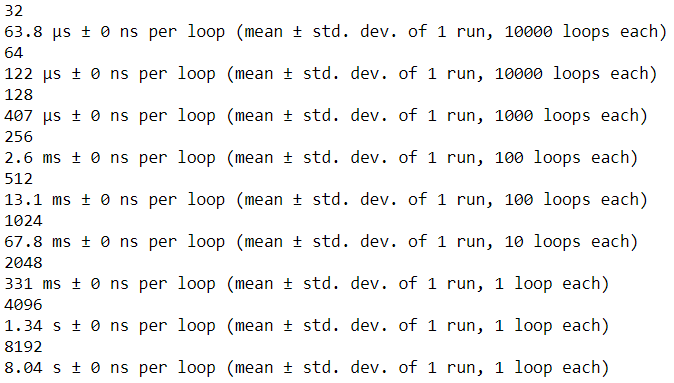
\includegraphics[width=0.8\textwidth]{fig1-1.PNG}
        \caption{Результаты analyze1}
        \label{fig:fig1-1}
\end{figure}  
\begin{figure}[H]
        \centering
        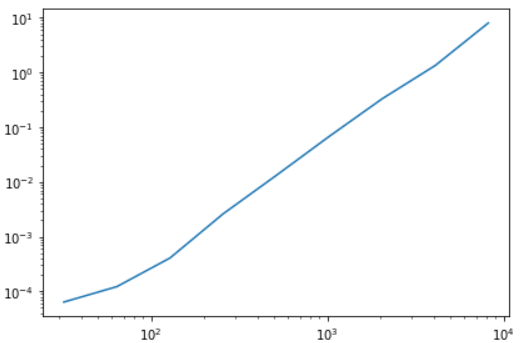
\includegraphics[width=0.8\textwidth]{fig1-2.PNG}
        \caption{График analyze1}
        \label{fig:fig1-2}
\end{figure}    

    Наклон полученного графика равен 2.2 (Рис.1.2), что не соотвествует нашим ожиданиям. Возможно так произошло из-за недостаточной выборки в массиве.
    
    Теперь посмотрим на функцию \texttt{analyze2}. Построим её график при тех же данных в массиве (Рис.1.3).
\begin{lstlisting}[caption=Получение результатов для analyze2]
       res2 = run_speed_test(ns, analyze2)
       plot_bests(ns, res2)
\end{lstlisting}
\begin{figure}[H]
        \centering
        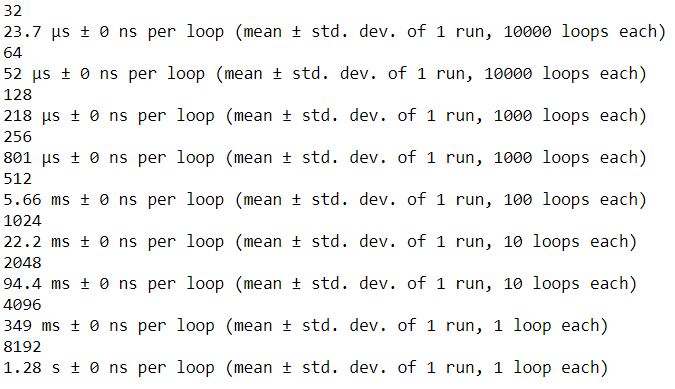
\includegraphics[width=0.8\textwidth]{fig1-3.PNG}
        \caption{Результаты analyze2}
        \label{fig:fig1-3}
\end{figure}  
\begin{figure}[H]
        \centering
        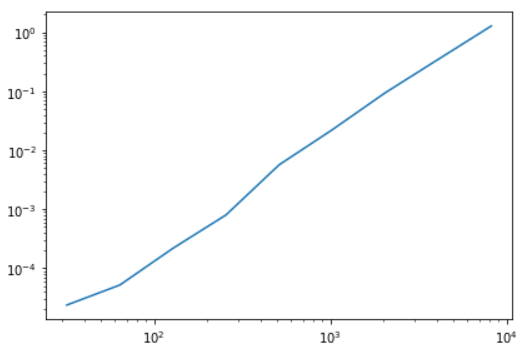
\includegraphics[width=0.8\textwidth]{fig1-4.PNG}
        \caption{График analyze2}
        \label{fig:fig1-4}
\end{figure} 

    Наклон данного графика равен 2.1 (Рис.1.4), что соотвествует нашим ожиданиям.  
    
    Также посмотрим на функцию \texttt{scipy.fftpack.dct} (Рис.1.5).
\begin{lstlisting}[caption=Получение результатов для scipy.fftpack.dct]
       import scipy.fftpack

       def scipy_dct(ys, freqs, ts):
           return scipy.fftpack.dct(ys, type=3)

       res3 = run_speed_test(ns, scipy_dct)
       plot_bests(ns, res3)
\end{lstlisting}
\begin{figure}[H]
        \centering
        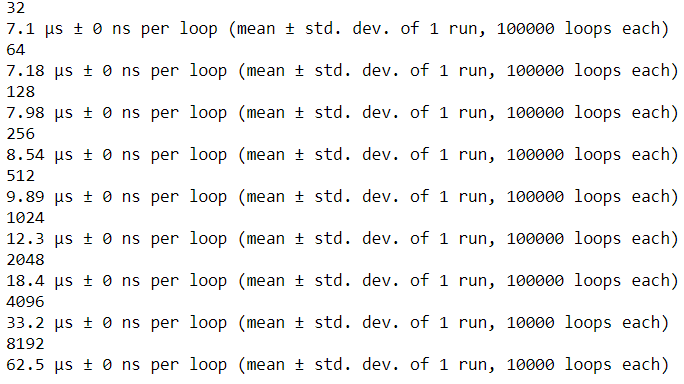
\includegraphics[width=0.8\textwidth]{fig1-5.PNG}
        \caption{Результаты scipy.fftpack.dct}
        \label{fig:fig1-5}
\end{figure}  
\begin{figure}[H]
        \centering
        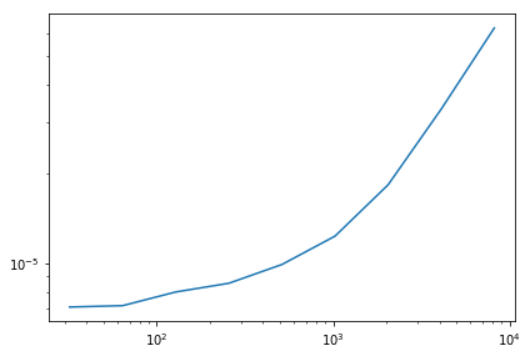
\includegraphics[width=0.8\textwidth]{fig1-6.PNG}
        \caption{График scipy.fftpack.dct}
        \label{fig:fig1-6}
\end{figure}     
     
     Данная функция работает еще быстрее. Как мы можем видеть на рис.1.6, её график изогнут, что означает, либо что мы еще не видели асимптотическое поведение, либо асимптотическое поведение не является простым показателем $n$. Ее выполнения пропорционально $n \log n$.
     
    Сравним полученные результаты (Рис.1.7).
\begin{figure}[H]
        \centering
        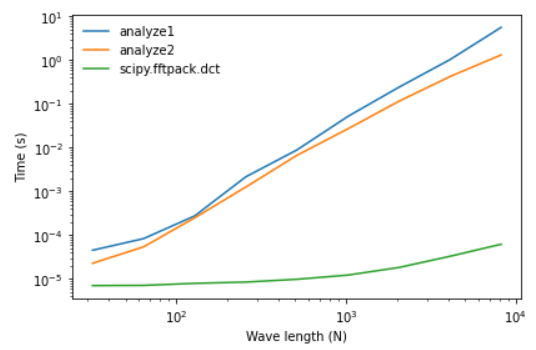
\includegraphics[width=0.8\textwidth]{fig1-7.PNG}
        \caption{Сравнение трех функций}
        \label{fig:fig1-7}
\end{figure}

\chapter{Упражнение 6.2}
\section{Алгоритм сжатия}
    Реализуем алгоритм сжатия звука с помощью ДКП. Применим его для записи музыки. 
    
    Алгоритм должен иметь следующие шаги:

    1. Разбиваем длинный сигнал на сегменты.
    
    2. Вычисляем ДКП каждого сегмента.
    
    3. Определяем частотные компоненты с такой амплитудой, что их не слышно, и удаляем их, сохраняя только оставшиеся частоты и амплитуды.
    
    4. При воспроизведении сигнала загружает частоты и амплитуды каждого сегмента и применяем обратное ДКП.

\section{Работа с коротким сегментом}
    Используем звук саксофона из предыдущей лабораторной и выделим из него небольшой сегмент.
\begin{lstlisting}[caption=Выделение сегмента]
       from thinkdsp import read_wave

       wave = read_wave('100475__iluppai__saxophone-weep.wav')
       segment = wave.segment(start=1.2, duration=0.5)
       segment.normalize()
       segment.make_audio()
\end{lstlisting}

    Теперь вычислим ДКП этого сегмента.
\begin{lstlisting}[caption=Приминение ДКП к сегменту]
       seg_dct = segment.make_dct()
       seg_dct.plot(high=4000)
       decorate(xlabel='Frequency (Hz)', ylabel='DCT')
\end{lstlisting}
\begin{figure}[H]
        \centering
        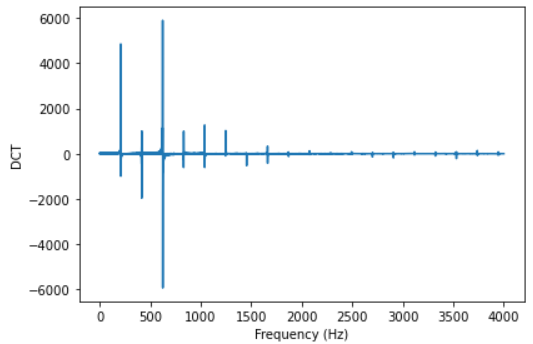
\includegraphics[width=0.8\textwidth]{fig2-1.PNG}
        \caption{ДКП сегмента}
        \label{fig:fig2-1}
\end{figure}    
       
    Как мы можем видеть на рис.2.1, только несколько частот имеют довольно большую амплитуду, остальные же близки к нулю.
    
    Зануляем слишком маленькие частоты, используя функцию \texttt{compress}.
\begin{lstlisting}[caption=Удаление неслышимых компонентов]
       def compress(dct, thresh=1):
           count = 0
           for i, amp in enumerate(dct.amps):
               if np.abs(amp) < thresh:
                   dct.hs[i] = 0
                   count += 1
            
           n = len(dct.amps)
           print(count, n, 100 * count / n, sep='\t')
    
       seg_dct = segment.make_dct()
       compress(seg_dct, thresh=10)
       seg_dct.plot(high=4000)
\end{lstlisting}
\begin{figure}[H]
        \centering
        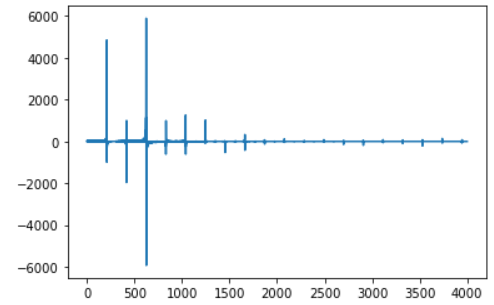
\includegraphics[width=0.8\textwidth]{fig2-2.PNG}
        \caption{ДКП фильтрованного сегмента}
        \label{fig:fig2-2}
\end{figure} 

    В результате применения \texttt{compress}, мы удалили около 93\% гармоник (Рис.2.2).

    Сравним звучание двух сегментов. На слух они одинаковые.

\section{Работа с длинным сегментом}    
    Чтобы сжать более длинный сегмент, мы можем сделать спектрограмму ДКП. Используем функцию \texttt{make\_dct\_spectrogram}, которая похожа на \texttt{make\_spectrogram}, но в ней используется ДКП.
\begin{lstlisting}[caption=Функция make\_dct\_spectrogram]
       from thinkdsp import Spectrogram

       def make_dct_spectrogram(wave, seg_length):
           window = np.hamming(seg_length)
           i, j = 0, seg_length
           step = seg_length // 2

           spec_map = {}

           while j < len(wave.ys):
               segment = wave.slice(i, j)
               segment.window(window)

               t = (segment.start + segment.end) / 2
               spec_map[t] = segment.make_dct()

               i += step
               j += step

           return Spectrogram(spec_map, seg_length)
\end{lstlisting}

    Теперь мы можем составить ДКП-спектрограмму и использовать сжатие для каждого сегмента.
\begin{lstlisting}[caption=Сжатие сегментов]
       spectro = make_dct_spectrogram(wave, seg_length=1024)
       for t, dct in sorted(spectro.spec_map.items()):
           compress(dct, thresh=0.2)
\end{lstlisting}

       В результате применения \texttt{compress}, мы удалили от 70 до 99\% гармоник у каждого сегмента.
       
       Теперь послушаем и сравним звучание до и после сжатия. В этом случае разница более заметная. Полученный звук напоминает немного искаженный оригинал.
       
\chapter{Упражнение 6.3}
    Воспользуемся блокнотом \texttt{phase.ipynb}, в котором исследуется влияние фазы на восприятие звука. Запустим примеры из него. Затем выберем другой сегмент звука и вновь поработаем с примерами.
 
\section{Пилообразный сигнал}      
    В начале мы возьмем пилообразный сигнал с частотой 500 и построим его спектр, а затем построим его угловую часть (Рис.3.1).
\begin{figure}[H]
        \centering
        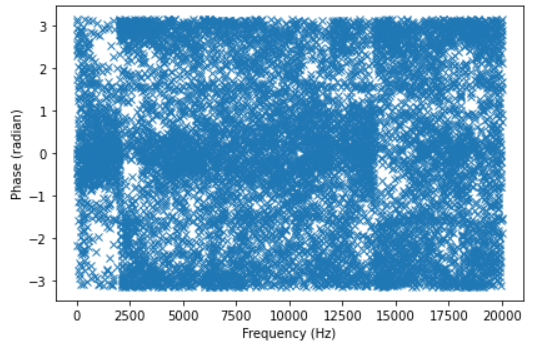
\includegraphics[width=0.8\textwidth]{fig3-1.PNG}
        \caption{Пилообразный сигнал. Угловая часть спектра}
        \label{fig:fig3-1}
\end{figure}

    При построении всех углов, мы получаем довольно запутанную картинку (Рис.3.1).
    
    Но если мы выберем только те частоты, где величина превышает порог, мы увидим, что в углах есть структура. Каждая гармоника смещена от предыдущей на доли радиана (Рис.3.2).
\begin{figure}[H]
        \centering
        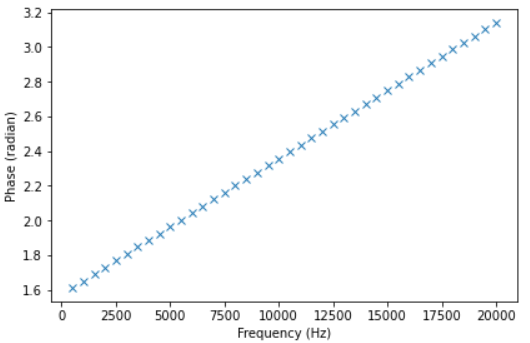
\includegraphics[width=0.8\textwidth]{fig3-2.PNG}
        \caption{Пилообразный сигнал. Угловая часть спектра с порогом}
        \label{fig:fig3-2}
\end{figure} 

    Теперь посмотрим, что произойдет, если мы установим все углы в ноль (Рис.3.3).
\begin{figure}[H]
        \centering
        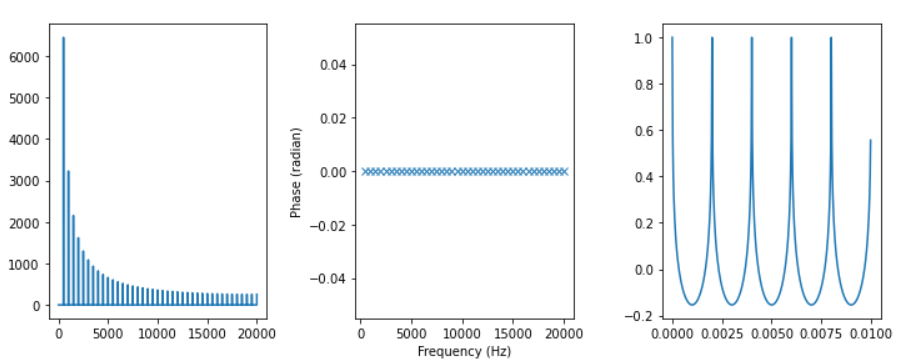
\includegraphics[width=0.8\textwidth]{fig3-3.PNG}
        \caption{Пилообразный сигнал. Нулевые углы}
        \label{fig:fig3-3}
\end{figure} 
    
    Амплитуда волны стала ниже, но это из-за способа нормализации волны, а не из-за изменений в фазовой структуре.  
    
    Теперь выполним поворот угла (Рис.3.4).
\begin{figure}[H]
        \centering
        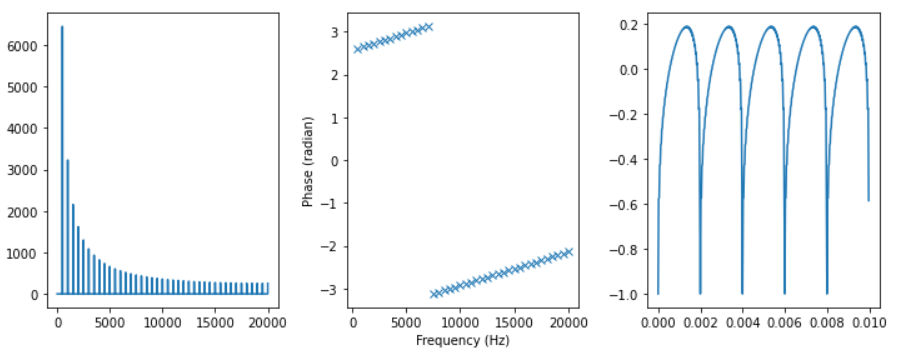
\includegraphics[width=0.8\textwidth]{fig3-4.PNG}
        \caption{Пилообразный сигнал. Поворот угла}
        \label{fig:fig3-4}
\end{figure}

    Также посмотрим, что произойдет, если мы установим для углов случайные значения (Рис.3.5).
\begin{figure}[H]
        \centering
        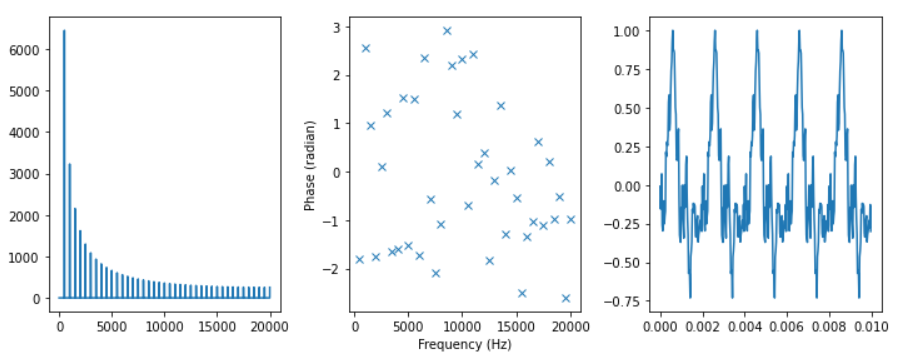
\includegraphics[width=0.8\textwidth]{fig3-5.PNG}
        \caption{Пилообразный сигнал. Случайные углы}
        \label{fig:fig3-5}
\end{figure}  

\section{Гобой} 
    Теперь поработаем с другими звуками. Воспользуемся записью гобоя. Выделим из неё новый сегмент. Снова построим спектр и его угловую часть (Рис.3.6).
\begin{lstlisting}[caption=Выделение сегмента]
       segment = wave.segment(start=1.0, duration=0.9)
\end{lstlisting}
\begin{figure}[H]
        \centering
        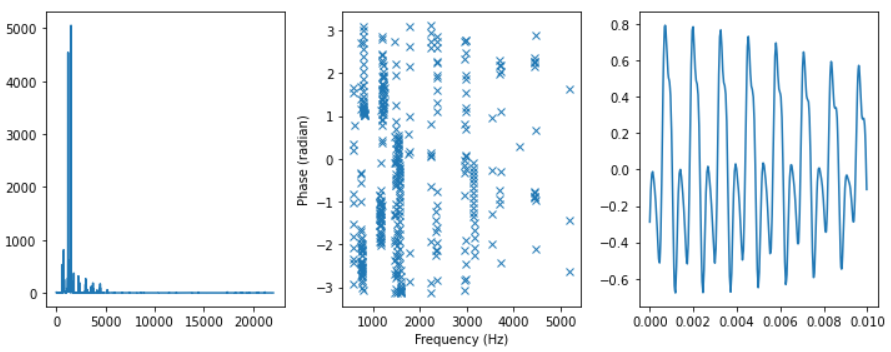
\includegraphics[width=0.8\textwidth]{fig3-6.PNG}
        \caption{Гобой. Угловая часть спектра}
        \label{fig:fig3-6}
\end{figure} 

    Теперь установим все углы в ноль (Рис.3.7).
\begin{figure}[H]
        \centering
        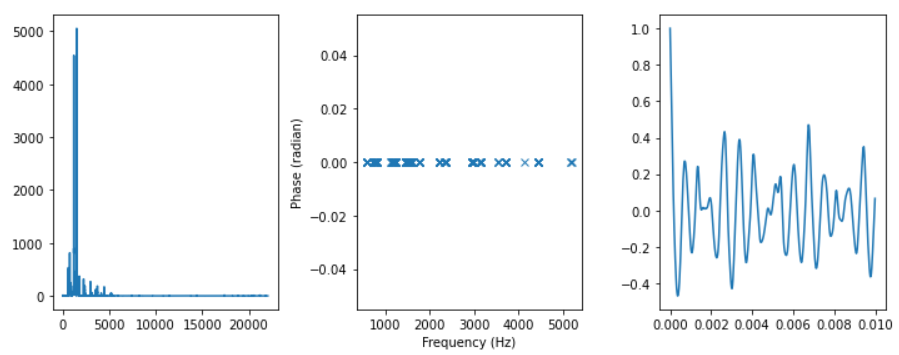
\includegraphics[width=0.8\textwidth]{fig3-7.PNG}
        \caption{Гобой. Нулевые углы}
        \label{fig:fig3-7}
\end{figure} 

    Изменение фазовой структуры, создает эффект «звона», когда громкость меняется со временем.
    
    Затем повернём угол на один радиан (Рис.3.8).    
\begin{figure}[H]
        \centering
        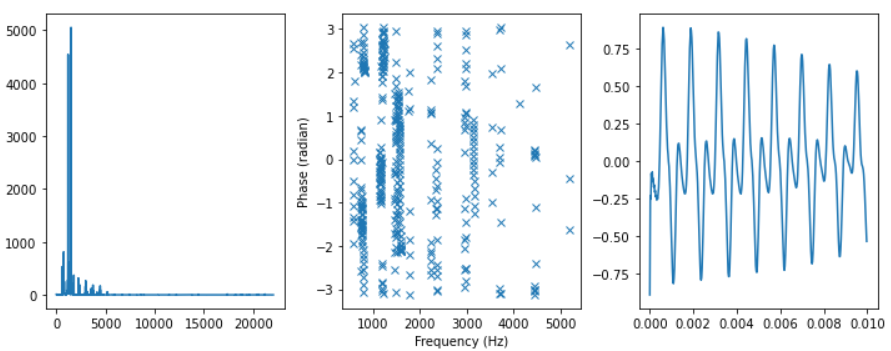
\includegraphics[width=0.8\textwidth]{fig3-8.PNG}
        \caption{Гобой. Поворот угла}
        \label{fig:fig3-8}
\end{figure}  
    
    Вращение углов не вызывает «звона».
    
    Далее установим случайные значения (Рис.3.9).
\begin{figure}[H]
        \centering
        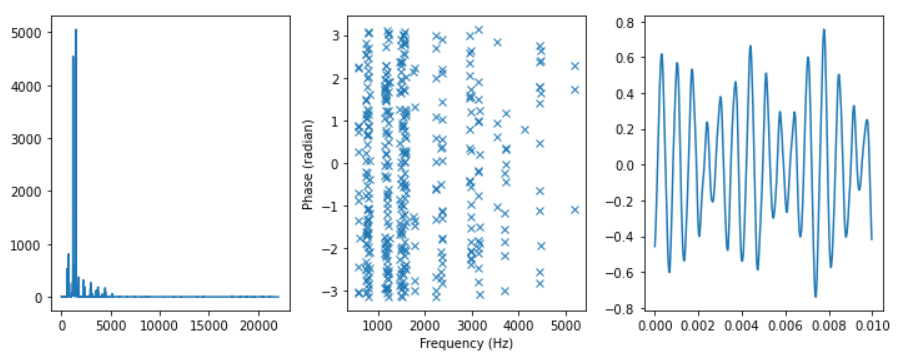
\includegraphics[width=0.8\textwidth]{fig3-9.PNG}
        \caption{Гобой. Случайные углы}
        \label{fig:fig3-9}
\end{figure}
    
    Случайный выбор углов вызывает некоторый звон и добавляет хриплости звуку. 
\section{Саксофон}  
    Проведя аналогичные исследования на саксофоне, мы получаем такие же результаты. Обнуление вызывает звон, вращение мало влияет, а использование случайных значений добавляет хрипы.
    
\section{Саксофон с удаленной основной частотой}
    Отличительной чертой саксофона от других звуков является то, что основная частота не является доминирующей. Попробуем её отфильтровать и посмотреть на результат.
    
    Обнуление (Рис.3.10).
\begin{figure}[H]
        \centering
        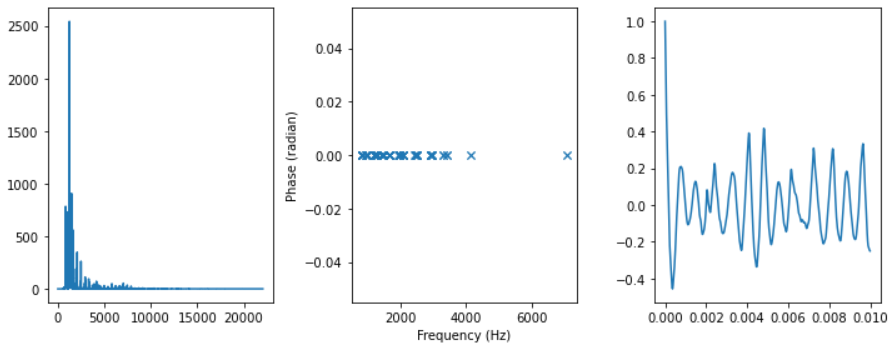
\includegraphics[width=0.8\textwidth]{fig3-10.PNG}
        \caption{Саксофон. Нулевые углы}
        \label{fig:fig3-10}
\end{figure}

    Поворот (Рис.3.11).
\begin{figure}[H]
        \centering
        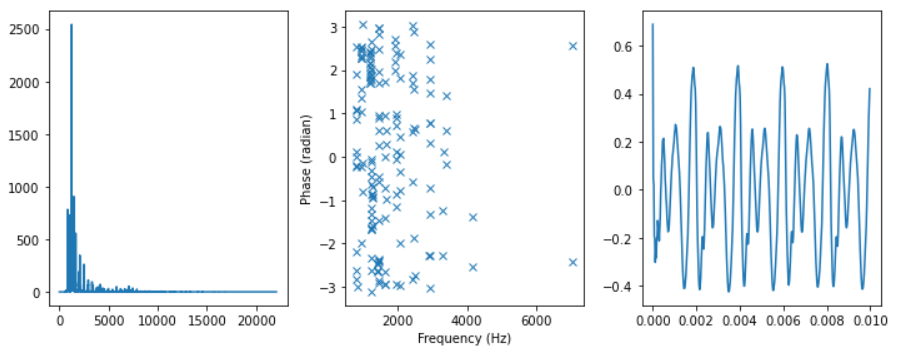
\includegraphics[width=0.8\textwidth]{fig3-11.PNG}
        \caption{Саксофон. Поворот угла}
        \label{fig:fig3-11}
\end{figure}

    Случайные значения (Рис.3.12).
\begin{figure}[H]
        \centering
        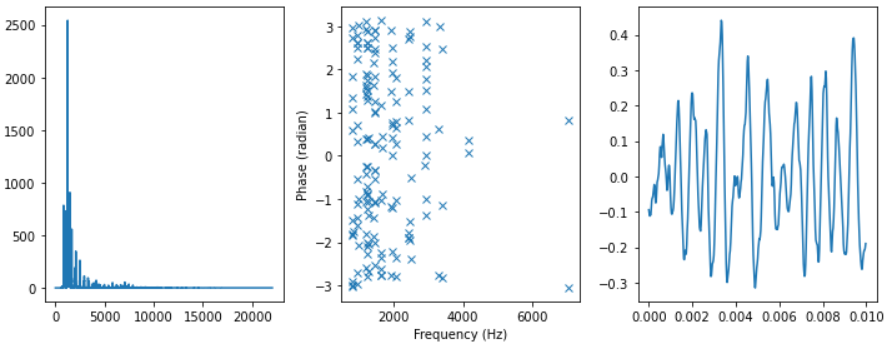
\includegraphics[width=0.8\textwidth]{fig3-12.PNG}
        \caption{Саксофон. Случайные углы}
        \label{fig:fig3-12}
\end{figure}  

    Таким образом, мы не слышим изменений в фазовой структуре звука, если он простой имеет простую гармоническую структуру и если гармоническая структура не изменилась.
    Возможным исключением являются звуки с низкой амплитудой у основной частоты.
    
\chapter{Выводы}
    В результате выполнения данной работы мы изучили дискретное косинусное преобразование и научились работать с ним. Также при помощи анализа разных звуков мы исследовали влияние фазы на восприятие звука.            
\end{document}